
The rocket, entitled RORO I, is a 8 feet (2.45 meters) rocket propelled by a M-class solid motor. The main requirements of the rocket are presented in Table \ref{table:se_topLevelR}.

\begin{table}[h!]
\centering
\begin{tabular}{|p{0.9\columnwidth}|}
\hline
    The rocket shall achieve an apogee of 10,000 ft (3048 meters).  \\ \hline
    The rocket shall have a static margin between 1 and 2 body-calibers \\ \hline
    The rocket shall carry a COTS barometric pressure altimeter with on-board storage as primary data source for altitude reporting.  \\ \hline
    The launch vehicle shall follow a "dual-event" recovery \\ \hline
    The rocket shall carry a minimum mass of 8.8 lb (4 kg) of payload. \\ \hline
    The rocket shall eject its nosecone at apogee. \\ \hline
    The rocket shall release a glider from the payload section at 10 seconds after apogee. \\ \hline

\end{tabular}
\caption{Top Level Requirements for the rocket}
\label{table:se_topLevelR}
\end{table}


\subsection{Design and Manufacturing}


The rocket is divided into 3 main sub-assemblies (Figure \ref{f:rocket_adnoted}:
\begin{enumerate}
    \item The nosecone - carrying avionics and an ejection system
    \item Upper Body - carrying the payload, the parachutes and the recovery electronics
    \item The Lower Body - containing logging avionics and the motor
\end{enumerate}
The concept of the rocket was well-thought to be easy to integrate and robust, considering the time constrains. The rocket separated in the middle, between the upper and lower body. This approach is very common in High Power Rocketry (HPR) and is considered a less risky approach.

The length as well as the diameter of the rocket were chosen in such a way to accommodate the payload which had a dimension constraint imposed by the competition (needed to be Cubesat standard).

Two important factors are important in a rocket: the dynamic stability and the static stability.




\begin{figure}[h!]
\centering
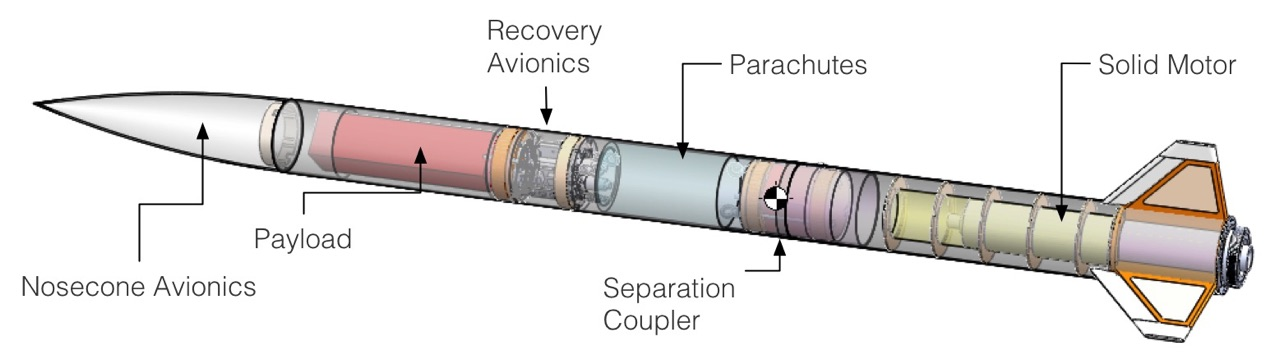
\includegraphics[width=0.5\textwidth]{img/rocket_sw_annotated.jpg}
\caption{The rocket with its main components}
\label{f:rocket_adnoted}
\end{figure}


\subsection{Recovery}

\subsection{Avionics}

%Podium session material
% Last 2 pictures (overall system explanation with arrows)

\subsection{Flight Tests-PATRICK}